% ROZDZIAŁ 13 — samodzielny rozdział do projektu teoria_miary
\chapter{Zamiana zmiennych w całce Lebesgue'a}
\label{ch:zamiana-zmiennych}

\section{Miary obrazowe: co właściwie zmienia się w całce?}
Niech $(X,\mathcal F,\mu)$ będzie przestrzenią z miarą, $(Y,\mathcal G)$
przestrzenią mierzalną, a $T:X\to Y$ odwzorowaniem mierzalnym.
\emph{Miara obrazowa} $T_\#\mu$ jest określona na $\mathcal G$ wzorem
$(T_\#\mu)(B)=\mu(T^{-1}(B))$. Nazwa ta nie oznacza, że
$\mu$ jest funkcją i można ją w zwykły sposób złożyć z $T$.

\begin{twierdzenie}[Całkowanie względem miary obrazowej]
\label{thm:pushforward-integral-13}
Niech $(X,\mathcal F,\mu)$ będzie przestrzenią z miarą,
$(Y,\mathcal G)$ przestrzenią mierzalną, a
$T:X\to Y$ odwzorowaniem $\mathcal F/\mathcal G$-mierzalnym.
Jeśli $h:Y\to[0,\infty]$ jest $\mathcal G$-mierzalna, to
\begin{equation}\label{eq:pushforward-13}
\int_Y h(y)\,\mathrm d(T_\#\mu)(y)
=\int_X h(T(x))\,\mathrm d\mu(x).
\end{equation}
Ta sama równość zachodzi dla funkcji $h:Y\to\mathbb C$
całkowalnych względem $T_\#\mu$.
\end{twierdzenie}
\begin{proof}
Dla $h=\chi_B$ obie strony są równe $\mu(T^{-1}(B))$.
Z liniowości wynika teza dla nieujemnych funkcji prostych.
Dla dowolnej $h\ge0$ wybieramy funkcje proste $h_n\uparrow h$;
$h_n\circ T\uparrow h\circ T$, więc dwukrotne zastosowanie
twierdzenia Beppo Leviego daje \eqref{eq:pushforward-13}.
Jeśli $h$ jest zespolona i całkowalna, poprzedni przypadek dla
$|h|$ dowodzi całkowalności $h\circ T$. Następnie rozdzielamy
części rzeczywiste i urojone oraz ich części dodatnie i ujemne.
\end{proof}

\begin{uwaga}
Równość \eqref{eq:pushforward-13} nie wymaga, aby $T$ było
różnowartościowe, ciągłe, różniczkowalne, ani nawet aby przestrzenie
$X,Y$ były topologiczne. Natomiast wzór z wyznacznikiem jakobianu,
który udowodnimy poniżej, wykorzystuje dodatkowo lokalną strukturę
przestrzeni euklidesowej i różnowartościowość $T$.
\end{uwaga}

\begin{przyklad}[Miara obrazu a rozkład zmiennej losowej]
Na $X=(0,1)$ z miarą Lebesgue'a rozważmy $T(x)=x^2$.
Dla $0\le t\le1$ mamy
$(T_\#\lambda_1)((0,t])=\sqrt t$; miara $T_\#\lambda_1$
ma zatem gęstość $y\mapsto(2\sqrt y)^{-1}$ na $(0,1)$.
W istocie wzór
$\int_{(0,1)}h(x^2)\,\mathrm d\lambda_1(x)
=\int_{(0,1)}h(y)/(2\sqrt y)\,\mathrm d\lambda_1(y)$
poznamy jako szczególny przypadek zamiany zmiennych.
Na razie wyprowadziliśmy równość miar na przedziałach $(0,t]$;
jednoznaczność miar skończonych na generującym układzie przedziałów
uzasadnia stwierdzenie o gęstości.
\end{przyklad}

\section{Zamiana liniowa i geometryczne znaczenie wyznacznika}

\begin{lemat}[Translacje, permutacje i ścinanie]
\label{lem:shear-13}
Niech $d\ge1$, $b\in\mathbb R^d$ i $E\subset\mathbb R^d$
będzie zbiorem borelowskim. Translacja $E\mapsto E+b$ zachowuje
miarę $\lambda_d$, podobnie jak dowolna permutacja współrzędnych.
Dla $d\ge2$, dowolnych
$i,j\in\{1,\ldots,d\}$, $i\ne j$, oraz $a\in\mathbb R$
miarę zachowuje także ścinanie postaci
\[
S(x_1,\ldots,x_d)=(x_1,\ldots,x_{j-1},
 x_j+a x_i,x_{j+1},\ldots,x_d).
\]
\end{lemat}
\begin{proof}
Niezmienniczość translacyjna została udowodniona w rozdziale 4.
Permutacje współrzędnych zachowują miarę prostokątów
półotwartych, zatem — przez jednoznaczność miary
$\sigma$-skończonej — wszystkich zbiorów borelowskich.
Dla ścinania ustalmy $d-1$ współrzędnych innych niż $x_j$.
W takim przekroju $S$ jest translacją zmiennej $x_j$
o stałą $a x_i$. Przekrój $S(E)$ jest więc translacją
odpowiedniego przekroju $E$. Ponieważ $S$ jest homeomorfizmem,
$S(E)$ jest borelowski. Twierdzenie Tonellego
\ref{thm:tonelli-12} zastosowane do funkcji charakterystycznych $\chi_E$ i $\chi_{S(E)}$
i niezmienniczość $\lambda_1$ dają równość ich miar.
\end{proof}

\begin{lemat}[Odwzorowania Lipschitzowskie zachowują zbiory zerowe]
\label{lem:lipschitz-null-13}
Niech $U\subset\mathbb R^d$ będzie otwarty, a
$F:U\to\mathbb R^d$ lokalnie Lipschitzowskie.
Jeżeli $N\subset U$ ma miarę Lebesgue'a zero, to
$\lambda_d(F(N))=0$ (w szczególności $F(N)$ jest mierzalny).
\end{lemat}
\begin{proof}
Zbiór $U$ można pokryć przeliczalnie domkniętymi sześcianami
$Q_j$ takimi, że każdy $Q_j$ zawiera się we wnętrzu
większego sześcianu położonego w $U$, na którym $F$
jest Lipschitzowska ze stałą $L_j<\infty$.
Takie pokrycie istnieje dzięki lokalnej własności
Lipschitza i przeliczalności bazy przestrzeni euklidesowej. Wystarczy rozważyć $N\cap Q_j$.
Dla ustalonego $j$ i $\varepsilon>0$ pokrywamy ten zbiór
przeliczalnie sześcianami $I_k$ o tak małych średnicach,
że leżą w odpowiednim otoczeniu $Q_j$ oraz
$\sum_k\lambda_d(I_k)<\varepsilon$.
Obraz $F(I_k)$ jest zawarty w sześcianie o boku
co najwyżej $2L_j\sqrt d$ razy bok $I_k$ (wokół
obrazu wybranego punktu $I_k$). Stąd
$\lambda_d^*(F(N\cap Q_j))\le C_d L_j^d\varepsilon$.
Przechodząc do $\varepsilon\downarrow0$, otrzymujemy
miarę zewnętrzną zero; zupełność miary Lebesgue'a
zapewnia mierzalność. Przeliczalna suma obrazów
$F(N\cap Q_j)$ jest więc zerowa.
\end{proof}

\begin{twierdzenie}[Liniowy wzór na objętość]
\label{thm:linear-change-13}
Jeżeli $A\in\mathrm{GL}(d,\mathbb R)$, $b\in\mathbb R^d$
i $E\subset\mathbb R^d$ jest borelowski, to
\begin{equation}\label{eq:linear-volume-13}
\lambda_d(AE+b)=|\det A|\lambda_d(E).
\end{equation}
Równość obowiązuje również dla dowolnego zbioru
$\lambda_d$-mierzalnego $E$, z wartościami w $[0,\infty]$.
\end{twierdzenie}
\begin{proof}
Mnożenie jednej współrzędnej przez $c\ne0$ mnoży miarę
przez $|c|$: w jednej zmiennej jest to skalowanie miary
Lebesgue'a, a w pozostałych stosujemy Tonellego.
Lemat~\ref{lem:shear-13} pokazuje, że operacje elementarne
polegające na dodaniu wielokrotności jednego wiersza do drugiego,
permutacji współrzędnych i skalowaniu pojedynczej współrzędnej
zmieniają miarę dokładnie przez moduł swego wyznacznika.
Eliminacja Gaussa przedstawia $A$ jako iloczyn skończenie
wielu takich macierzy. Kolejne zastosowanie ustalonych wzorów
i multiplikatywność wyznacznika dają \eqref{eq:linear-volume-13}
dla zbiorów borelowskich.

Macierz $A$ i jej odwrotność są globalnie Lipschitzowskie.
Z lematu~\ref{lem:lipschitz-null-13} wynika, że odwzorowanie lokalnie
Lipschitzowskie przenosi zbiory zerowe na zbiory miary zero.
Każdy zbiór Lebesgue'a-mierzalny różni się od zbioru borelowskiego
co najwyżej na podzbiorze borelowskiego zbioru zerowego;
zatem $AE+b$ jest mierzalny, a jego miara jest wyznaczona
przez część borelowską. To daje rozszerzenie na miarę zupełną.
\end{proof}

\begin{uwaga}[Wymiar ma znaczenie]
Twierdzenie~\ref{thm:linear-change-13} wymaga
macierzy kwadratowej nieosobliwej. W przypadku odwzorowań
$\mathbb R^m\to\mathbb R^n$, $m\ne n$, pojawiają się
inne wielkości (jakobiany wymiarowe, miary Hausdorffa),
które wprowadzimy w geometrycznej części skryptu.
\end{uwaga}

\section{Lokalna deformacja sześcianu}

\begin{lemat}[Oszacowanie obrazu małego sześcianu]
\label{lem:small-cube-13}
Niech $U\subset\mathbb R^d$ będzie otwarty, a
$\Phi:U\to\mathbb R^d$ odwzorowaniem klasy $C^1$.
Niech $x_0\in U$ oraz załóżmy, że
$A=D\Phi(x_0)$ jest odwracalna.
Dla $r>0$ oznaczmy $Q_r=[-r,r]^d$ i przyjmijmy
$x_0+Q_r\subset U$. Istnieje funkcja $\delta(r)\to0$
przy $r\downarrow0$ taka, że dla dostatecznie małych $r$
\begin{equation}\label{eq:cube-est-13}
(1-\delta(r))^d|\det A|\lambda_d(Q_r)
\le \lambda_d(\Phi(x_0+Q_r))
\le(1+\delta(r))^d|\det A|\lambda_d(Q_r).
\end{equation}
W szczególności iloraz miary obrazu i objętości sześcianu
dąży do $|\det D\Phi(x_0)|$.
\end{lemat}
\begin{proof}
Wprowadzamy normę maksimum $\|z\|_\infty$ w $\mathbb R^d$
i funkcję $H(z)=A^{-1}(\Phi(x_0+z)-\Phi(x_0))$.
Zachodzi $H(0)=0$ i $DH(0)=I$.
Niech $R(z)=H(z)-z$. Z ciągłości $DH$ wynika, że
\[
\delta(r):=\sup_{z\in Q_r}\|DR(z)\|_{\infty\to\infty}
\longrightarrow0.
\]
Dla $z,w\in Q_r$ twierdzenie o przyrostach skończonych
wzdłuż odcinka $[z,w]$ daje
$\|R(z)-R(w)\|_\infty\le\delta(r)\|z-w\|_\infty$,
a po podstawieniu $w=0$ dostajemy
$\|R(z)\|_\infty\le\delta(r)r$.
Zatem $H(Q_r)\subseteq Q_{(1+\delta(r))r}$.

Dla $y\in Q_{(1-\delta(r))r}$ rozważmy
$T_y(z)=y-R(z)$ na pełnej, domkniętej przestrzeni
metrycznej $Q_r$. Funkcja ta odwzorowuje $Q_r$ w siebie,
gdyż $\|T_y(z)\|_\infty\le(1-\delta)r+\delta r=r$,
i jest zwężeniem o stałej $\delta(r)<1$.
Twierdzenie o punkcie stałym Banacha (iteracja
$z_{n+1}=T_y(z_n)$ i oszacowanie geometryczne różnic)
daje $z\in Q_r$ z $T_y(z)=z$, czyli $H(z)=y$.
Wynika stąd drugie zawieranie
$Q_{(1-\delta(r))r}\subseteq H(Q_r)$.
Po zastosowaniu $A$ i translacji otrzymujemy
\[
\Phi(x_0)+A Q_{(1-\delta)r}
\subseteq\Phi(x_0+Q_r)
\subseteq\Phi(x_0)+A Q_{(1+\delta)r}.
\]
Miary skrajnych zbiorów liczymy za pomocą
\eqref{eq:linear-volume-13}; monotoniczność miary
daje \eqref{eq:cube-est-13}.
\end{proof}

\begin{uwaga}
W dowodzie nie użyto nieudowodnionego wzoru o zamianie zmiennych,
lecz tylko przypadku liniowego i twierdzenia o punkcie stałym.
Co więcej, na zbiorze zwartym, na którym $D\Phi$ jest ciągła
i odwracalna, parametry $\delta(r)$ można dobrać
\emph{jednostajnie} względem środka sześcianu, o ile sześciany
leżą w ustalonym otwartym otoczeniu tego zbioru.
Istotne są tu jednostajna ciągłość $D\Phi$ i ograniczoność
normy $(D\Phi)^{-1}$ na rozważanym zbiorze zwartym.
\end{uwaga}

\section{Główne twierdzenie o zamianie zmiennych}

\begin{twierdzenie}[Zamiana zmiennych dla dyfeomorfizmu $C^1$]
\label{thm:change-variables-13}
Niech $U,V\subset\mathbb R^d$ będą otwarte i niech
$\Phi:U\to V$ będzie dyfeomorfizmem klasy $C^1$
(tzn. bijekcją, dla której $\Phi$ i $\Phi^{-1}$
są klasy $C^1$). Wtedy:
\begin{enumerate}[label=\textup{(\roman*)}]
\item dla każdego zbioru Lebesgue'a-mierzalnego $E\subset U$
zbiór $\Phi(E)$ jest Lebesgue'a-mierzalny i
\begin{equation}\label{eq:change-sets-13}
\lambda_d(\Phi(E))=\int_E |\det D\Phi(x)|\,
\mathrm d\lambda_d(x);
\end{equation}
\item dla każdej Lebesgue'a-mierzalnej
$f:V\to[0,\infty]$ zachodzi
\begin{equation}\label{eq:change-main-13}
\int_V f(y)\,\mathrm d\lambda_d(y)
=\int_U f(\Phi(x))|\det D\Phi(x)|\,
\mathrm d\lambda_d(x);
\end{equation}
\item ta sama równość zachodzi dla funkcji
$f:V\to\mathbb C$ całkowalnych względem $\lambda_d$.
\end{enumerate}
\end{twierdzenie}
\begin{proof}
\emph{Krok 1. Miara obrazu dla zbiorów borelowskich.}
Dla borelowskiego $E\subset U$ określamy
$\tau(E)=\lambda_d(\Phi(E))$. Jest to miara na
$\mathcal B(U)$, ponieważ $\Phi$ jest homeomorfizmem:
obrazy zbiorów borelowskich są borelowskie w $V$, a obrazy
rozłącznych zbiorów są rozłączne. Określamy drugą miarę
$\rho(E)=\int_E J(x)\,\mathrm d\lambda_d(x)$,
gdzie $J(x)=|\det D\Phi(x)|$. Funkcja $J$ jest dodatnia
i ciągła; obie miary są $\sigma$-skończone, ponieważ
$U$ jest przeliczalną sumą zwartych podzbiorów,
a obrazy tych zwartych zbiorów są zwarte.

\emph{Krok 2. Równość na sześcianach.}
Niech $Q\subset U$ będzie domkniętym sześcianem.
Dzielimy go na $n^d$ przystających, domkniętych
sześcianów $Q_{n,j}$, $1\le j\le n^d$, o rozłącznych wnętrzach.
Na mocy lematu~\ref{lem:lipschitz-null-13} obraz brzegu
każdego $Q_{n,j}$ ma miarę zero. Zatem
$\tau(Q)=\sum_j\tau(Q_{n,j})$.
Wybieramy środek $x_{n,j}$ sześcianu $Q_{n,j}$.
Ponieważ $Q\Subset U$, funkcje $D\Phi$ i
$(D\Phi)^{-1}$ są na zwartym zbiorze $Q$ odpowiednio
jednostajnie ciągłe i ograniczone; stąd w oszacowaniach
wszystkich $Q_{n,j}$ można przyjąć jeden parametr
$\delta_n\to0$, niezależny od $j$.
Oszacowanie z lematu~\ref{lem:small-cube-13},
jednostajne względem tych środków, prowadzi do
\[
(1-\delta_n)^d\sum_jJ(x_{n,j})\lambda_d(Q_{n,j})
\le\tau(Q)\le
(1+\delta_n)^d\sum_jJ(x_{n,j})\lambda_d(Q_{n,j}),
\qquad\delta_n\to0.
\]
Sumy $\sum_jJ(x_{n,j})\lambda_d(Q_{n,j})$ zbiegają
do $\int_QJ(x)\,\mathrm d\lambda_d(x)$ jako sumy Riemanna
funkcji ciągłej na zwartym sześcianie. Otrzymujemy
$\tau(Q)=\rho(Q)$. Ta sama równość dotyczy wnętrza
sześcianu i półotwartego sześcianu, bo ich brzegi
oraz obrazy tych brzegów mają miarę zero.

\emph{Krok 3. Równość miar na $\mathcal B(U)$.}
Niech $\mathcal P$ będzie rodziną wszystkich półotwartych
sześcianów diadycznych, których domknięcia zawierają się
w $U$, wraz ze zbiorem pustym. Dwa sześciany diadyczne
albo są rozłączne, albo jeden zawiera się w drugim.
Zatem $\mathcal P$ jest układem typu $\pi$:
dwa sześciany w tej samej siatce diadycznej albo są
rozłączne, albo identyczne, a sześciany w siatkach
o różnych skalach są rozłączne lub jeden zawiera się
w drugim. Dokładniej używamy półotwartych sześcianów
$\prod_{j=1}^d[k_j2^{-n},(k_j+1)2^{-n})$,
$n\in\mathbb N_0$, $k_j\in\mathbb Z$, których domknięcia
są zawarte w $U$. Rodzina ta jest przeliczalna,
pokrywa $U$ i generuje
$\mathcal B(U)$: dla każdego $x\in U$ oraz otwartego
otoczenia $W\subset U$ punktu $x$ można wybrać
sześcian diadyczny $Q$ z $x\in Q$ i $\overline Q\subset W$.
Na każdym $C\in\mathcal P$ mamy
$\tau(C)=\rho(C)<\infty$. Aby poprawnie zastosować
argument $\pi$--$\lambda$, dla ustalonego takiego $C$
rozważamy dwie \emph{skończone} miary
$\tau_C(E)=\tau(E\cap C)$ oraz
$\rho_C(E)=\rho(E\cap C)$ na $\mathcal B(U)$.
Na $\mathcal P$ są równe, ponieważ $E\cap C\in\mathcal P$,
a z twierdzenia $\pi$--$\lambda$ wynika
$\tau(E\cap C)=\rho(E\cap C)$ dla dowolnego
$E\in\mathcal B(U)$. Wreszcie numerujemy sześciany
$C_1,C_2,\dots$ pokrywające $U$ i rozłączamy je przez
$D_1=C_1$, $D_j=C_j\setminus\bigcup_{i<j}C_i$.
Dla każdego borelowskiego $E\subset U$ równość miar
na $E\cap D_j$ wynika ze skończonej addytywności
równości na $E\cap C_j$ i $E\cap C_j\cap C_i$
(lub z rozdzielenia przez wcześniejsze sześciany).
Po zsumowaniu po $j$ dostajemy
$\tau(E)=\rho(E)$. To rozpisanie jest potrzebne:
rodzina sześcianów $\mathcal P$ sama nie zawiera
na ogół rosnącego wyczerpania $U$.

\emph{Krok 4. Uzupełnienie i przejście do całek.}
Ponieważ $\Phi$ oraz $\Phi^{-1}$ są lokalnie
Lipschitzowskie, lemat~\ref{lem:lipschitz-null-13}
pokazuje, że obrazy i przeciwobrazy zbiorów
$\lambda_d$-zerowych są zerowe. Każdy zbiór Lebesgue'a-
mierzalny różni się od borelowskiego na zbiorze zerowym,
a więc tożsamość $\tau(E)=\rho(E)$ rozciąga się na
wszystkie Lebesgue'a-mierzalne $E\subset U$; daje to (i).

Wzór (ii) sprawdzamy najpierw dla funkcji $f=\chi_B$,
$B\subset V$ mierzalnego: jego lewa strona to
$\lambda_d(B)$, a prawa, na mocy (i), to
$\int_{\Phi^{-1}(B)}J(x)\,\mathrm d\lambda_d(x)$,
co jest równe $\lambda_d(B)$.
Następnie korzystamy z liniowości dla funkcji prostych
i z twierdzenia Beppo Leviego dla funkcji nieujemnych.
W przypadku funkcji zespolonej całkowalnej stosujemy
(ii) do $|f|$, aby zapewnić całkowalność prawej strony,
a następnie rozkładamy $f$ na cztery części nieujemne.
\end{proof}

\begin{wniosek}[Zamiana na mierzalnym podzbiorze]
\label{cor:change-subdomain-13}
Niech $U,V\subset\mathbb R^d$ będą otwarte,
a $\Phi:U\to V$ dyfeomorfizmem klasy $C^1$.
Niech $E\subset U$ będzie zbiorem Lebesgue'a-mierzalnym,
a $g:\Phi(E)\to[0,\infty]$ funkcją mierzalną.
Wtedy, przy oznaczeniu
$J(x)=|\det D\Phi(x)|$, zachodzi
\[
\int_{\Phi(E)}g(y)\,\mathrm d\lambda_d(y)
=\int_E g(\Phi(x))J(x)\,\mathrm d\lambda_d(x).
\]
Ta sama równość zachodzi dla zespolonych funkcji $g$
całkowalnych na $\Phi(E)$.
\end{wniosek}
\begin{proof}
Przedłużamy $g$ przez zero na $V\setminus\Phi(E)$
i stosujemy poprzednie twierdzenie.
\end{proof}

\begin{uwaga}[Skąd bierze się moduł?]
Gdy $\det D\Phi<0$, odwzorowanie zmienia orientację,
lecz miara Lebesgue'a jest nieujemna. Z tego powodu
w formule występuje $|\det D\Phi|$, nie sam wyznacznik.
W całkowaniu form różniczkowych bez modułu uwzględnia się
orientację i otrzymuje inną regułę.
\end{uwaga}

\section{Przykłady: współrzędne biegunowe, walcowe i sferyczne}

\begin{przyklad}[Współrzędne biegunowe]
\label{ex:polar-13}
Rozważmy $\Phi:(0,\infty)\times(0,2\pi)\to\mathbb R^2$,
$\Phi(r,\theta)=(r\cos\theta,r\sin\theta)$.
Jest to dyfeomorfizm na płaszczyznę bez dodatniej
półosi poziomej i punktu początkowego, czyli na
$\mathbb R^2\setminus\{(x,0):x\ge0\}$.
Jego macierz pochodnej ma kolumny
$(\cos\theta,\sin\theta)^T$ i
$(-r\sin\theta,r\cos\theta)^T$, stąd
$\det D\Phi(r,\theta)=r$. Usunięta półprosta ma
$\lambda_2$-miarę zero. Dlatego dla każdej
mierzalnej funkcji $f:\mathbb R^2\to[0,\infty]$
\begin{equation}\label{eq:polar-13}
\int_{\mathbb R^2}f(x,y)\,\mathrm d\lambda_2(x,y)
=\int_{(0,2\pi)}\left(\int_{(0,\infty)}
 f(r\cos\theta,r\sin\theta)r\,\mathrm d\lambda_1(r)\right)
\mathrm d\lambda_1(\theta).
\end{equation}
Kolejność całkowania uzasadnia twierdzenie Tonellego.
Dla $f=\chi_{\{x^2+y^2<R^2\}}$ otrzymujemy
$\lambda_2(B(0,R))=\int_{(0,2\pi)}\int_{(0,R)}r\,
\mathrm d\lambda_1(r)\,\mathrm d\lambda_1(\theta)=\pi R^2$.
\end{przyklad}

\begin{center}
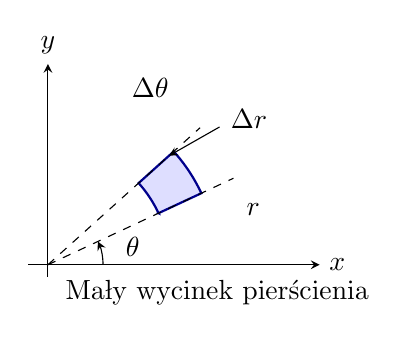
\begin{tikzpicture}[scale=1.0,>=stealth]
\draw[->] (-0.25,0)--(3.45,0) node[right] {$x$};
\draw[->] (0,-0.15)--(0,2.55) node[above] {$y$};
\filldraw[fill=blue!13,draw=blue!55!black,thick]
(25:1.55) -- (25:2.15) arc[start angle=25,end angle=42,radius=2.15]
-- (42:1.55) arc[start angle=42,end angle=25,radius=1.55] -- cycle;
\draw[dashed] (0,0)--(25:2.6);
\draw[dashed] (0,0)--(42:2.6);
\draw[->] (0.7,0) arc[start angle=0,end angle=25,radius=0.7];
\node at (12:1.1) {$\theta$};
\node[anchor=west] at (2.2,1.85) {$\Delta r$};
\draw[->] (2.18,1.75)--(42:2.07);
\node at (60:2.6) {$\Delta\theta$};
\node at (15:2.7) {$r$};
\node[anchor=west] at (0.1,-0.35) {Mały wycinek pierścienia};
\end{tikzpicture}
\end{center}
\noindent
Dla małych przyrostów $\Delta r$ i $\Delta\theta$ pole
zaznaczonego wycinka jest w pierwszym przybliżeniu
$r\,\Delta r\,\Delta\theta$. Jest to geometryczna intuicja
za jakobianem $r$; ścisłym uzasadnieniem jest jednak
twierdzenie~\ref{thm:change-variables-13}.

\begin{przyklad}[Współrzędne walcowe]
Dla $r>0$, $\theta\in(0,2\pi)$, $z\in\mathbb R$
połóżmy $\Psi(r,\theta,z)=(r\cos\theta,r\sin\theta,z)$.
Wyznacznik jej macierzy pochodnej wynosi $r$.
Po odrzuceniu półpłaszczyzny miary Lebesgue'a zero
otrzymujemy dla każdej mierzalnej
$f:\mathbb R^3\to[0,\infty]$
\[
\begin{aligned}
\int_{\mathbb R^3}f(x,y,z)\,\mathrm d\lambda_3(x,y,z)
&=\int_{\mathbb R}\int_{(0,2\pi)}\int_{(0,\infty)}
 f(r\cos\theta,r\sin\theta,z)r\,
\mathrm d\lambda_1(r)\,\mathrm d\lambda_1(\theta)
\,\mathrm d\lambda_1(z).
\end{aligned}
\]
Równość obowiązuje również dla zespolonych funkcji
$f\in L^1(\mathbb R^3,\lambda_3)$.
\end{przyklad}

\begin{przyklad}[Współrzędne sferyczne]
Dla $r>0$, $\vartheta\in(0,\pi)$, $\varphi\in(0,2\pi)$
rozważmy
$\Psi(r,\vartheta,\varphi)=
(r\sin\vartheta\cos\varphi,
 r\sin\vartheta\sin\varphi,r\cos\vartheta)$.
Bezpośrednie obliczenie wyznacznika daje
$|\det D\Psi|=r^2\sin\vartheta$.
Po odrzuceniu odpowiedniej półpłaszczyzny i osi,
które mają miarę zero, otrzymujemy dla każdej mierzalnej
$f:\mathbb R^3\to[0,\infty]$
\begin{align*}
\int_{\mathbb R^3}f(x)\,\mathrm d\lambda_3(x)
&=\int_{(0,\infty)}\int_{(0,\pi)}\int_{(0,2\pi)}
 f(\Psi(r,\vartheta,\varphi))r^2\sin\vartheta\,
 \mathrm d\lambda_1(\varphi)\,\mathrm d\lambda_1(\vartheta)
 \,\mathrm d\lambda_1(r).
\end{align*}
Ta sama równość zachodzi dla zespolonych funkcji
$f\in L^1(\mathbb R^3,\lambda_3)$.
Dla kuli $B(0,R)$ daje to $\lambda_3(B(0,R))=4\pi R^3/3$.
\end{przyklad}

\section{Obrazy miar posiadających gęstości}
\begin{twierdzenie}[Transformacja gęstości]
\label{thm:density-transform-13}
Niech $U,V\subset\mathbb R^d$ będą otwarte,
a $\Phi:U\to V$ dyfeomorfizmem klasy $C^1$.
Niech $w:U\to[0,\infty]$ będzie mierzalna i
niech $\mu$ będzie miarą na zbiorach Lebesgue'a-mierzalnych
$E\subset U$, określoną wzorem
$\mu(E)=\int_Ew(x)\,\mathrm d\lambda_d(x)$.
Wtedy dla każdego mierzalnego $B\subset V$
\[
(\Phi_\#\mu)(B)=\int_B
w(\Phi^{-1}(y))|\det D\Phi^{-1}(y)|\,
\mathrm d\lambda_d(y).
\]
\end{twierdzenie}
\begin{proof}
Z definicji miary obrazowej mamy
$(\Phi_\#\mu)(B)=\int_{\Phi^{-1}(B)}w(x)\,
\mathrm d\lambda_d(x)$.
Stosujemy twierdzenie~\ref{thm:change-variables-13}
do dyfeomorfizmu $\Phi^{-1}:V\to U$ oraz funkcji
$h:U\to[0,\infty]$, określonej przez
$h(x)=\chi_{\Phi^{-1}(B)}(x)w(x)$.
Ponieważ
$h(\Phi^{-1}(y))=\chi_B(y)w(\Phi^{-1}(y))$,
otrzymujemy
\[
\int_{\Phi^{-1}(B)}w(x)\,\mathrm d\lambda_d(x)
=\int_B w(\Phi^{-1}(y))|\det D\Phi^{-1}(y)|
\,\mathrm d\lambda_d(y).
\]
W obu całkach iloczyn $0\cdot\infty$ interpretujemy
jako $0$, zgodnie z konwencją całkowania funkcji
nieujemnych o wartościach rozszerzonych.
\end{proof}

\begin{przyklad}[Rozkład jednostajny i kwadratowanie]
Jeśli $X$ ma rozkład jednostajny na $(0,1)$ i
$Y=X^2$, to $Y$ ma gęstość na $\mathbb R$ daną wzorem
\[
p_Y(y)=
\begin{cases}
\dfrac{1}{2\sqrt y},&0<y<1,\\
0,&y\notin(0,1).
\end{cases}
\]
To dokładnie miara obrazowa rozważana na początku rozdziału.
Nie ma potrzeby zakładać, że sam $X$ jest określony
na $(0,1)$: wystarczy, aby jego rozkład był jednostajny.
\end{przyklad}

\section{Założenia, które naprawdę są potrzebne}
\begin{przyklad}[Dlaczego nie wolno pomijać różnowartościowości]
Dla $\Phi:\mathbb R\to\mathbb R$, $\Phi(x)=x^2$,
nie istnieje globalna odwrotność. Gdyby bez dodatkowych
poprawek użyć wzoru z jakobianem na całej prostej, dla
$f=\chi_{(0,1)}$ otrzymalibyśmy po prawej stronie
$\int_{(-1,1)}2|x|\,\mathrm d\lambda_1(x)=2$,
zaś po lewej $\int_{(0,1)}1\,\mathrm d\lambda_1(y)=1$.
Rozbieżność wynika z dwukrotnego liczenia punktów obrazu.
Dla nieiniektywnych odwzorowań właściwym narzędziem
jest wzór z krotnością włókien, a w większej ogólności
wzór na pole powierzchni (późniejszy rozdział).
\end{przyklad}

\begin{przyklad}[Wymagana regularność]
Z samej różnowartościowości i ciągłości $\Phi$ nie wynika
wzór z pochodną. Na przykład istnieją ściśle rosnące
homeomorfizmy przedziału, których pochodna znika
prawie wszędzie (homeomorfizmy osobliwe).
Przy takiej funkcji całka pochodnej nie daje długości obrazu.
Nie wystarczy więc samo istnienie pochodnej prawie wszędzie:
w odpowiedniej wersji uogólnionej potrzebne są dodatkowe
własności, np. absolutna ciągłość w wymiarze jeden.
\end{przyklad}

\section{Podsumowanie}
Wzór na całkę względem miary obrazowej jest czysto
mierzalny. Natomiast wyznacznik jakobianu opisuje
lokalną zmianę objętości pod dyfeomorfizmem $C^1$.
Dowód przeszedł od macierzy elementarnych do lokalnych
sześcianów, a następnie do równości miar i funkcji
mierzalnych. Formuły biegunowe i sferyczne wynikają
z jednego twierdzenia, a nie z odrębnych reguł rachunkowych.
